\chapter{Анализ методов повышения качества на границе проводной и беспроводной сети} \label{chapt1}


\section{Анализ перспектив развития беспроводных сетей} \label{sect1_0}
В этом разделе мы рассмотрим тендеции развития мобильной связи.
Согласно отчета Ericsson \cite{ericsson} число абонентов мобильной связи во всем мире выросло примерно на 8 процентов в годовом исчислении в 1 квартале 2013 года. Число абонентов мобильной широкополосной связи выросло еще быстрее за этот период в размере 45 процентов в годовом исчислении, достигнув около 1,7 миллиарда. Количество данных, передаваемых каждым усстройством, также неуклонно продолжает расти. Около 50 процентов всех проданных мобильных телефонов в 1 квартале 2013 были смартфонами. Все эти факторы привели к удвоению мобильного трафика между 1 кварталом 2012 и 1 кварталом 2013 года. 

В 1 квартале 2013 года общее количесво мобильных устройств превысило 6,4 миллиарда. К концу 2018 года ожидается 9,1 миллиард обслуживаемых устройств. 

Глобальное количество обслуживаемых широкополосных устройств достигло в 1 квартал 2013 года 1,7 миллиарда и к концу 2018 года достигнет 7 миллиардов (рис. \ref{img1:mob1}). Основными устройствами широкополосного доступа есть и будут смартфоны. Мобильный широкополосный доступ получит большую долю от общей широкополосной связи на многих рынках, дополняя XDSL в определенных сегментах и заменяя его в других. 

Количество обслуживаемых мобильных устройств, таких как мобильные ПК, мобильные роутеры, планшеты, которые используют большой экран, увеличится с 300 млн в 2012 году до 850 млн в 2018 году, что привысит число абонентов фиксированной широкополосной связи (рис. \ref{img1:mob2}).
Общее количество смартфонов достигло в 2012 году 1,2 млрд и, как ожидается, вырастет до 4,5 млрд в 2018 году. На сегодняшний день основным мобильным устройством является базовый телефон. Проникновение смартфонов будет быстро увеличиваться, в то время как, по оценкам, количество обслуживаемых базовых телефонов останется высоким, медленно снижаясь с 5 млрд сегодня до 4 млрд в 2018 году. Это связано с тем что базовые телефоны будут продолжать находится в нижнем сегменте продаваемых абонентских устройств.

\pgfplotsset{width=15cm, height=10cm, compat=1.3}
\begin{figure} [h]
  \center
\begin{tikzpicture}
\pgfkeys{ /pgf/number format/.cd,
        use comma,
        1000 sep={}}
\pgfkeys{/pgfplots/legend pos=north west}
\begin{axis}[
legend cell align=left,
cycle list name=mark list,
xlabel=Год,
ylabel=Количесво абонентов/линий (млн)
]

\addplot coordinates
{(2009,4200) (2010,4850) (2011,5500) (2012,6000) (2013,6500) (2014,7000) (2015,7500) (2016,8000) (2017,8500) (2018,9000)};

\addplot coordinates
{(2009,300) (2010,600) (2011,1000) (2012,1500) (2013,2100) (2014,3000) (2015,3700) (2016,4800) (2017,5800) (2018,7000)};

\addplot coordinates
{(2009,500) (2010,525) (2011,550) (2012,575) (2013,600) (2014,625) (2015,650) (2016,675) (2017,700) (2018,725)};

\addplot coordinates
{(2009,50) (2010,140) (2011,230) (2012,320) (2013,410) (2014,500) (2015,590) (2016,680) (2017,770) (2018,860)};
\legend{Мобильные абоненты, Мобильные широкополосные линии, Проводные широкополосные линии, Мобильные ПК/планшеты/мобильные роутеры}
\end{axis}
\end{tikzpicture}
\caption{Стационарные и мобильные обслуживаемые устройства, 2009-2018 \cite{ericsson}}
  \label{img1:mob1}
\end{figure}


\pgfplotsset{width=15cm, height=10cm, compat=1.3}
\begin{figure} [h]
  \center
\begin{tikzpicture}
\pgfkeys{ /pgf/number format/.cd,
        use comma,
        1000 sep={}}
\pgfkeys{/pgfplots/legend pos=north west}



\begin{axis}[stack plots=y,/tikz/ybar,
legend cell align=left,
cycle list name=mark list,
xlabel=Год,
ylabel=Количесво абонентов (млн)
]
\addplot coordinates
{(2010,4466) (2011,4711) (2012,4741) (2013,4639) (2014,4483) (2015,4289) (2016,4099) (2017,3926) (2018,3763)};
\addplot coordinates
{(2010,522) (2011,836) (2012,1247) (2013,1781) (2014,2363) (2015,2944) (2016,3504) (2017,4017) (2018,4493)};
\addplot coordinates
{(2010,166) (2011,238) (2012,308) (2013,386) (2014,467) (2015,554) (2016,647) (2017,745) (2018,846)};

\legend{Функциональный/Базовый телефон, Смартфон, Мобильный ПК/Маршрутизатор/Планшет}
\end{axis}
\end{tikzpicture}
\caption{Прогноз развития беспроводных сетей по устройствам \cite{ericsson}}
  \label{img1:mob2}
\end{figure}


\clearpage


На рис. \ref{img1:mob3} иллюстрирован отчет по количеству обслуживаемых мобильных устройств различными технологиями: LTE, WCDMA/HSPA, GSM/EDGE, TD-SCDMA, CDMA и другими. Технология LTE, которая развернута и представлена во всех регионах, в 2018 году составит 2 млрд устройств. Эти устройства будут представлять лидирующую долю от обшего количества устройств. Быстрый переход на более совершенные технологии в развитых странах, означает что мировое количество абонентов GSM/EDGE будет снижаться после 2012-2013 годов. Глобально, GSM/EDGE будет продолжать играть ведущую роль с точки зрения числа абонентов до послених лет прогнозного периода. Это связано с тем что новые менее обеспеченные пользователи, вероятно будут использовать самые дешевые мобильные устройства и технологии мобильной связи. Кроме этого требуется время для обновления установленной базы мобильных устройств.


\pgfplotsset{width=15cm, height=10cm, compat=1.3}
\begin{figure} [h]
  \center
\begin{tikzpicture}
\pgfkeys{ /pgf/number format/.cd,
        use comma,
        1000 sep={}}
\pgfkeys{/pgfplots/legend pos=north west}
\begin{axis}[stack plots=y,/tikz/ybar,
legend cell align=left,
cycle list name=mark list,
xlabel=Год,
ylabel=Количесво абонентов (млн)
]
\addplot coordinates
{(2010,64) (2011,54) (2012,37) (2013,34) (2014,35) (2015,35) (2016,35) (2017,29) (2018,23)};
\addplot coordinates
{(2010,497) (2011,532) (2012,545) (2013,537) (2014,525) (2015,514) (2016,503) (2017,485) (2018,473)};
\addplot coordinates
{(2010,21) (2011,51) (2012,94) (2013,149) (2014,199) (2015,229) (2016,231) (2017,223) (2018,201)};
\addplot coordinates
{(2010,3904) (2011,4182) (2012,4311) (2013,4263) (2014,4060) (2015,3717) (2016,3240) (2017,2696) (2018,2117)};
\addplot coordinates
{(2010,668) (2011,956) (2012,1245) (2013,1648) (2014,2148) (2015,2710) (2016,3321) (2017,3874) (2018,4336)};
\addplot coordinates
{(2010,0) (2011,9) (2012,64) (2013,176) (2014,346) (2015,583) (2016,920) (2017,1381) (2018,1953)};

\legend{Other Technology, CDMA, TD-SCDMA, GSM/EDGE, WCDMA/HSPA, LTE}
\end{axis}
\end{tikzpicture}
\caption{Прогноз развития беспроводных сетей по технологиям \cite{ericsson}}
  \label{img1:mob3}
\end{figure}


Мобильный трафик изменяется. На рис. \ref{img1:mob4} изображена устойчивая тенденция роста трафика данных с некоторыми сезонными колебаниями. Это показывает, что мобильные данные абонентов сильно вырастут. Ведущую роль в увеличении общего количества трафика данных сыграло непрерывное увеличение среднего объема данных передаваемое и принимаемое с каждого устройства.


В 2013 году, как и ожидалось, общий мобильный трафик продолжил тенденцию удвоения каждый год. Трафик от мобильных ПК доминирует в большинстве регионов. Тем не менее, трафик смартфонов растет быстрее за счет увеличения числа устройств. В последние годы прогнозного периода, трафик данных будет довольно равномерно разделен между мобильными телефонами, с одной стороны, планшетами, мобильными маршрутизаторами и мобильными ПК с другой (рис. \ref{img1:mob5}). Мобильный трафик будет расти значительно быстрее, чем фиксированный трафик данных в течение прогнозируемого периода. Тем не менее, в абсолютном объеме, трафик в фиксированных сетях останется доминирующим за тот же период (рис. \ref{img1:mob6}). 

\clearpage

\pgfplotsset{
    /pgfplots/area legend/.style={%
        /pgfplots/legend image code/.code={%
            \fill[##1] (0cm,-0.1cm) rectangle (0.6cm,0.1cm);
        }%
    },
}



\usetikzlibrary{patterns}

\begin{figure} [!h]
  \center
%\includegraphics[width=0.95\textwidth]{ericsson/mob5.png}
\begin{tikzpicture}
\begin{axis}[
legend cell align=left,
cycle list name=linestyles*,
area legend,
axis x line=bottom,
axis y line=left,
legend style={at={(0.03,0.97)},anchor=north west},
xlabel=Год,
ylabel=Общий трафик (Петабайт),
ymin=0,
ybar,
bar width=5pt,
Axis Style,
    xtick={
        2007, 2007.25, 2007.5, 2007.75,
        2008, 2008.25, 2008.5, 2008.75,
        2009, 2009.25, 2009.5, 2009.75,
        2010, 2010.25, 2010.5, 2010.75,
        2011, 2011.25, 2011.5, 2011.75,
        2012, 2012.25, 2012.5, 2012.75,
        2013, 2013.25, 2013.5, 2013.75
    },
    xticklabels={
        $\tiny \begin{array}{c}Q1 \\ 2007\end{array}$, $\tiny \begin{array}{c}Q2 \end{array}$, $\tiny \begin{array}{c}Q3\end{array}$, $\tiny \begin{array}{c}Q4\end{array}$,
        $\tiny \begin{array}{c}Q1 \\ 2008\end{array}$, $\tiny \begin{array}{c}Q2\end{array}$, $\tiny \begin{array}{c}Q3\end{array}$, $\tiny \begin{array}{c}Q4\end{array}$,
        $\tiny \begin{array}{c}Q1 \\ 2009\end{array}$, $\tiny \begin{array}{c}Q2\end{array}$, $\tiny \begin{array}{c}Q3\end{array}$, $\tiny \begin{array}{c}Q4\end{array}$,
        $\tiny \begin{array}{c}Q1 \\ 2010\end{array}$, $\tiny \begin{array}{c}Q2\end{array}$, $\tiny \begin{array}{c}Q3\end{array}$, $\tiny \begin{array}{c}Q4\end{array}$,
        $\tiny \begin{array}{c}Q1 \\ 2011\end{array}$, $\tiny \begin{array}{c}Q2\end{array}$, $\tiny \begin{array}{c}Q3\end{array}$, $\tiny \begin{array}{c}Q4\end{array}$,
        $\tiny \begin{array}{c}Q1 \\ 2012\end{array}$, $\tiny \begin{array}{c}Q2\end{array}$, $\tiny \begin{array}{c}Q3\end{array}$, $\tiny \begin{array}{c}Q4\end{array}$,
        $\tiny \begin{array}{c}Q1 \\ 2013\end{array}$, $\tiny \begin{array}{c}Q2\end{array}$, $\tiny \begin{array}{c}Q3\end{array}$, $\tiny \begin{array}{c}Q4\end{array}$
    }
]
\addplot [pattern color=red!50, draw=black, pattern=north west lines] coordinates
{(2007,70) (2007.25,75) (2007.5,80) (2007.75,85) (2008,90) (2008.25,100) (2008.5,110) (2008.75,120) (2009,130) (2009.25,140) (2009.5,145) (2009.75,150) (2010,155) (2010.25,160) (2010.5,160) (2010.75,160) (2011,160) (2011.25,160) (2011.5,160) (2011.75,160) (2012,160) (2012.25,160) (2012.5,160) (2012.75,160) (2013,160) (2013.25,0)}
\closedcycle;

\addplot [pattern color=blue!50, draw=black, pattern=north east lines] coordinates
{(2007,3) (2007.25,5) (2007.5,8) (2007.75,10) (2008,13) (2008.25,15) (2008.5,20) (2008.75,30) (2009,50) (2009.25,80) (2009.5,120) (2009.75,160) (2010,180) (2010.25,220) (2010.5,250) (2010.75,320) (2011,390) (2011.25,400) (2011.5,480) (2011.75,560) (2012,760) (2012.25,840) (2012.5,1000) (2012.75,1280) (2013,1520) (2013.25,0)}
\closedcycle;

\legend{Речь, Данные}
\end{axis}



\end{tikzpicture}
  \caption{Глобальный общий трафик передачи речи и данных в мобильных сетях, 2007-2013 \cite{ericsson}}
  \label{img1:mob4}
\end{figure}


\begin{figure} [!h]
  \center
%\includegraphics[width=0.95\textwidth]{ericsson/mob5.png}
\begin{tikzpicture}
\begin{axis}[
legend cell align=left,
stack plots=y,
%area style,
enlarge x limits=false,
area legend,
axis x line=bottom,
axis y line=left,
domain=0:1,
legend style={at={(0.03,0.97)},anchor=north west},
xlabel=Год,
ylabel=Общий месячный трафик ($10^{18}$ байт)
]
\addplot[pattern color=red!50, draw=black, pattern=north west lines] coordinates
{(2010,0.1) (2011,0.1) (2012,0.2) (2013,0.2) (2014,0.25) (2015,0.25) (2016,0.27) (2017,0.3) (2018,0.3)}
\closedcycle;
\addplot[
    pattern=vertical lines,
    pattern color=green!50,
    draw=black,
] coordinates
{(2010,0.1) (2011,0.3) (2012,0.5) (2013,1.1) (2014,1.7) (2015,2.7) (2016,3.7) (2017,5.5) (2018,7.7)}
\closedcycle;
\addplot[
    pattern=horizontal lines,
    pattern color=blue!50,
    %pattern color=black!50!white,
    draw=black,] coordinates
{(2010,0.1) (2011,0.3) (2012,0.5) (2013,0.7) (2014,1.5) (2015,2.3) (2016,3) (2017,4) (2018,6)}
\closedcycle;
\legend{Речь, Данные мобильных телефонов, Данные мобильных ПК/планшетов/мобильных роутеров}
\end{axis}
\end{tikzpicture}
  \caption{Глобальный трафик передачи речи и данных в мобильных сетях, 2010-2018 \cite{ericsson}}
  \label{img1:mob5}
\end{figure}


\begin{figure} [!h]
  \center
%\includegraphics[width=0.95\textwidth]{ericsson/mob5.png}
\begin{tikzpicture}
\begin{axis}[
legend cell align=left,
stack plots=y,
%area style,
enlarge x limits=false,
area legend,
axis x line=bottom,
axis y line=left,
domain=0:1,
legend style={at={(0.03,0.97)},anchor=north west},
xlabel=Год,
ylabel=Общий месячный трафик ($10^{18}$ байт)
]
\addplot[pattern color=blue!50, draw=black, pattern=vertical lines] coordinates
{(2010,20) (2011,25) (2012,30) (2013,40) (2014,50) (2015,65) (2016,85) (2017,110) (2018,145)}
\closedcycle;


\end{axis}
\end{tikzpicture}
  \caption{Глобальный трафик в фиксированных сетях, 2010-2018 \cite{ericsson}}
  \label{img1:mob6}
\end{figure}


Такие сервисы как социальные сети и сервисы с картинками и видео, являются драйверами роста мобильного трафика. В результате объем трафика возростет к концу 2018 года в 12 раз. Рост трафика частично связан с размером экрана пользовательского устройства. Разрешение экрана также является фактором, влияющим на трафик. Современные смартфоны приблизились к уровню качества ПК экранов. В среднем один мобильный ПК генерирует приблизительно в 5 раз больше трафика чем смартфон. К концу 2012 года, средний мобильный ПК генерирует около 2,5 Гб трафика в месяц, по сравнению со средним смартфоном - 450 МБ в месяц. К концу 2018 года, по оценкам, в среднем, мобильный ПК будет генерировать около 11 Гб в месяц и смартфон около 2 Гбайт. Следует отметить, что существуют большие различия в пользовательских шаблонах между различными сетями, рынками и пользователями.

Рост числа абонентов в широкополосной мобильной связи, является мощным стимулом роста для мобильного трафика. С увеличением числа пользователей, увеличивается количество устройств подключенных к сети, таких как смартфоны, планшеты, мобильные ПК, мобильные роутеры, електронные книги и камеры.  Самым быстрорастущим сегментом в мобильном трафике является видео. Увеличение использования контента приводит в постоянный рост количество доступного контента, а так же к лучшим сетевым скоростям, которые приходят с развитием HSPA и LTE. Рост размеров экранов устройств и разрешения экранов, также будут драйвером увеличения мобильного трафика, так как они позволят смотреть видео высокой четкости, а в дальнейшем и сверх высокой. 

Сервисы с потоковым видео так же показали высокую популярность. Люди используют эти сервисы на всех типах устройств. Так же видеоконференции при использовании мобильных устройств, будут стимулировать рост видео трафика в мобильных сетях. Сегодня видео составляет крупнейший сегмент трафика данных в мобильных сетях, и, как ожидается, будет расти примерно на 60 процентов в год вплоть до конца 2018 года, на этот момент, по прогнозам, объем видео трафика составит около половины от общего глобального трафика (рис. \ref{img1:mob7}).

Потоковая музыка приобретает все большую популярность и аудио как ожидается, будет расти с годовым темпом роста около 50 процентов. Существует высокая степень неопределенности в прогнозе на аудио трафик на данном этапе, так как он очень сильно зависит от того, как сервисы потоковой музыки будут развиваться в ближайшие годы.
Просмотр веб-страниц и социальных сетей будет каждый составлять около 10 процентов от общего объема трафика данных в 2018 году.
Приход новых типов устройств или информационного контента способного быстро изменить трафик, в настоящее время, не считается значительным. Кроме того, будет широкая вариация между сетями с различными профилями устройств, например, некоторые из них будут с доминированием PC в то время как другие будут способствовать использованию смартфонов. Трафик также будет меняться между рынками из-за различий в доступности контента и прав. 

\definecolor{RYB3}{RGB}{190, 186, 218}
\definecolor{RYB1}{RGB}{141, 211, 199}
\begin{figure} [!h]
  \center
%\includegraphics[width=0.95\textwidth]{ericsson/mob5.png}
\begin{tikzpicture}
\begin{axis}[
legend cell align=left,
stack plots=y,
%area style,
enlarge x limits=false,
area legend,
axis x line=bottom,
axis y line=left,
domain=0:1,
legend style={at={(0.03,0.97)},anchor=north west},
xlabel=Год,
ylabel=Общий месячный трафик ($10^{18}$ байт)
]
\addplot[pattern color=blue!50, draw=black, pattern=vertical lines] coordinates
{(2010,0.05) (2012,0.06) (2013,0.1) (2014,0.15) (2015,0.2) (2016,0.3) (2017,0.4) (2018,0.5)}
\closedcycle;

\addplot[pattern color=red!50, draw=black, pattern=horizontal lines] coordinates
{(2010,0.05) (2012,0.4) (2013,0.9) (2014,1.5) (2015,2.3) (2016,3.5) (2017,5.2) (2018,7)}
\closedcycle;

\addplot[pattern color=blue!50, draw=black, pattern=north west lines] coordinates
{(2010,0.03) (2012,0.05) (2013,0.07) (2014,0.1) (2015,0.15) (2016,0.2) (2017,0.25) (2018,0.3)}
\closedcycle;

\addplot[pattern color=green!50, draw=black, pattern=fivepointed stars] coordinates
{(2010,0.05) (2012,0.12) (2013,0.2) (2014,0.4) (2015,0.6) (2016,0.9) (2017,1.1) (2018,1.6)}
\closedcycle;

\addplot[pattern color=orange!100, draw=black, pattern=dots] coordinates
{(2010,0.04) (2012,0.1) (2013,0.15) (2014,0.2) (2015,0.4) (2016,0.6) (2017,0.9) (2018,1.1)}
\closedcycle;

\addplot[pattern color=RYB1!100, draw=black, pattern=grid] coordinates
{(2010,0.04) (2012,0.1) (2013,0.17) (2014,0.23) (2015,0.3) (2016,0.4) (2017,0.5) (2018,0.7)}
\closedcycle;

\addplot[pattern color=RYB3!100, draw=black, pattern=sixpointed stars] coordinates
{(2010,0.04) (2012,0.1) (2013,0.17) (2014,0.25) (2015,0.35) (2016,0.5) (2017,0.7) (2018,0.9)}
\closedcycle;

\addplot[pattern color=blue!50, draw=black, pattern=north east lines] coordinates
{(2010,0.05) (2012,0.1) (2013,0.2) (2014,0.5) (2015,1) (2016,1.4) (2017,1.7) (2018,2)}
\closedcycle;

\legend{Файлы в общем доступе, Видео, Аудио, Веб сайты, Социальные сети, Скачивание и обновление ПО, Шифрованный трафик, Другое}
\end{axis}
\end{tikzpicture}
  \caption{Глобальный трафик разбитый по приложениям, 2010-2018 \cite{ericsson}}
  \label{img1:mob7}
\end{figure}



Когда пользователь меняет свой телефон на смартфон, он все равно продолжает пользоваться голосовыми и текстовыми сообщениями. Пользователи склонны к развитию привычки использования приложения в течении некоторого времени после того как они открыли новое приложение или сервис. Рекомендации пользователей, семьи, рекламы и магазинов для новых и трендовых приложений играют значительную роль. 

Со временем, пользователи, как правило, используют более современные услуги, которые ставят более высокие требования к возможностям устройства. Сегодня пользователи смартфонов, которые подключаются к сервисам с музыкой и потоковым видео уже потребляют больше, чем 2 Гб трафика в месяц в среднем. Это в четыре раза больше потребления среднего пользователя со смартфоном. Во многих магазинах, легальные потоковые сервисы для музыки и для видео набирают популярность. При достаточном контенте и правильном уровне цен эти услуги демонстрируют высокие темпы популяризации.

Прогнозы для каждой категории мобильных данных показывают значительный рост до 2018 года. Наибольший прирост ожидается от видео трафика, и, по оценкам, составит около половины всего мобильного трафика данных к концу прогнозируемого периода. Видео трафик, в том числе и часть зашифрованного и трафик совместного использования файлов,скорее всего, представит большую часть всего мобильного трафика данных к 2018 году.



%Вследствие всего выше перечисленного, потоковый трафик набирает все большую популярность и обеспечение 





\section{Конвергенция фиксированный и мобильных сетей} \label{sect1_1}
Как мы уже рассмотрели, мобильные сети и трафик меняется и большинство операторов сталкиваются с такими проблемами, как насыщение рынка, ценовое давление и необходимостью снижения эксплуатационных затрат.
Операторы фиксированной связи отмечают снижение доходов от предоставления традиционных услуг передачи речи и потерю доли дохода от наземных линий доступа. Для операторов продолжилась эпоха слияний и поглощений, для вендоров - слияний, поглощений и поиска взаимовыгодных альянсов (когда продуктовые линейки и маркетинговые возможности компаний взаимовыгодно дополняют друг друга). По ряду технических и административных причин продолжился рост влияния на рынке компаний - системных интеграторов. Основными причинами этого является расширение абонентской базы мобильной связи и развитие услуг передачи речи через IP (Voice over IP - VoIP). В краткосрочной перспективе доходы провайдеров услуг фиксированной связи будут расти за счет доходов от услуг передачи данных IP, в частности, от широкополосных услуг для домашнего сектора.  Многие операторы мобильной связи столкнулись с проблемой замедления темпов роста базы частных абонентов и вынуждены были уделить серьезное внимание повышению доходности в других областях, таких как услуги передачи данных и услуги на корпоративном рынке. В качестве одного из решений перечисленных проблем, является концепция конвергенции фиксированной и мобильной связи - Fixed Mobile Convergence (FMC), способствующая, с одной стороны, повышению доходов операторов, с другой - удовлетворению растущих требований конечных заказчиков, которые ориентированы на мобильные и IP-технологии. FMC будет способствовать принятию сетей нового поколения \cite{FMC}, в которых весь коммуникационный трафик использует IP.
Существует несколько способов предоставления FMC услуг, некоторые из которых более технологически интегрированы, чем другие. Есть менее развитые формы FMC использующие двухрежимные телефоны сотовый/Wi-Fi, которые не имеют функции handover или имею эту функцию, но не используют ее для передачи речи или для доступа к широкополосной сети в домашних условиях. Также существуют услуги соединяющие мобильную и фиксированную сеть, но в которых технологически не происходит конвергенция, такие как предложение единого голосового и почтового ящика поверх фиксированных и мобильных сетей.
Концепция конвергенции фиксированных и мобильных сетей широка, многогранна и развивается. 


Концепция FMC состоит из трех основных уровней: конвергенция сетей; конвергенция услуг; конвергенция приложений \cite{IMS}.
\begin{enumerate}
\item Сетевая конвергенция. На уровне сетевой конвергенции обеспечивается снижение эксплуатационных расходов за счет конвергенции различных сетей фиксированной и мобильной связи в единую магистральную сеть IP/MPLS, поддерживающую широкий спектр методов доступа: традиционную телефонию, DSL, выделенные каналы, беспроводные сети (WLAN) и сети радиодоступа (RAN) в сетях операторов мобильной связи.
Конвергенция магистрали и сетей доступа является наиболее очевидным и проработанным этапом процесса слияния фиксированных и мобильных платформ.
Эта концепция охватывает, в том числе и передачу значительных объемов речевого трафика по той же магистрали IP, по которой доставляются широкополосные данные, услуги GPRS и UMTS, - так называемый перевод транзитного трафика на сеть IP. 
Для операторов мобильной связи конвергентные сети обычно начинаются переводом трафика сервиса коротких сообщений (SMS), сервиса мультимедийных сообщеий (MMS) и сетей сигнализации с традиционных платформ в сеть IP - это ускоряет конвергенцию протоколов сигнализации с IP. При передаче трафика сети радиодоступа 2.5G и 3G через оптимизированную сеть доступа IP сетевая конвергенция обеспечивает глубину проникновения вплоть до сети доступа оператора мобильной связи.


\item Конвергенция услуг. На уровне конвергенции услуг выполняются функции управления сессиями. Именно этот уровень делает возможным развертывание высокодоходных услуг нового поколения на основе IP, таких как мобильный доступ к данным, проведение аудио- и видеоконференций, передача речи и мгновенный обмен сообщениями. Осведомленность о каждой сессии и контроль над ними обеспечивает доступность услуги на любом абонентском терминале и через любой метод доступа, позволяя переключаться между различными типами доступа без негативного воздействия на активные сессии. Кроме того, именно уровень конвергенции услуг гарантирует, что любой услуге IP выделяются соответствующие сетевые ресурсы, а любая услуга должным образом тарифицируется. Один из основных показателей функциональности конвергентной платформы, является обеспечение непрерывности услуги при пересечении границы между фиксированной и мобильной сетью.
Концепция непрерывности услуги достаточно специфична для каждой из областей - передачи речи, передачи данных и передачи мультимедийного трафика. 
Однако такие технологии, как конвергентные речевые устройства (телефоны, смартфоны, КПК, ноутбуки и т. д.), архитектуры конвергенции речевых сессий и протоколы конвергенции сессий данных являются связующим звеном между фиксированными и мобильными платформами. Другим ключевым элементом является осведомленность платформы, через которую доставляется услуга, о передаваемых сессиях и ее способность выполнять специфические действия по применению политик вне зависимости от местоположения участников сессии и их метода доступа, будь то проводной доступ по xDSL или мобильные данные в среде LTE. Конвергенция услуг - это тот основополагающий уровень, который в конечном счете обеспечивает потребителям удобство пользования услугами, выполняя незаметную для абонентов передачу сессий данных и речи между наземным и беспроводным широкополосными доменами. При этом сеть динамически адаптирует свои политики по выделению ресурсов и обеспечению качества обслуживания, учитывая факт мобильности терминала и то, в какой среде передачи терминал находится в данный момент.

\item Конвергенция приложений. Уровень конвергенции приложений включает собственно услуги, с которыми операторы выходят на рынок и которые они собираются рекламировать в качестве конечного продукта. В частности, непрерывные услуги передачи данных, предоставляемые через любую сеть доступа, речевые услуги для предприятий с двухрежимными терминалами (например, Wi-Fi/GSM) и т. д. Конвергенция приложений - это процесс доставки приложений через множество различных сред передачи в формате, учитывающем различие скоростей доступа, которые эти среды обеспечивают. Домен конвергентных приложений поддерживается и обеспечивается в основном функциональностью протокола SIP, учитывающего мобильность абонентов и динамичность их состояния (регистрации) на соответствующих серверах. Как один из примеров конвергентных приложений можно назвать одновременную доставку видеопотока на терминал 3G и персональный компьютер через сеть распространения контента из одного и того же сервисного центра. Более обобщенно, конвергенция приложений - это предоставление потребителям услуг передачи речи , данных и видео через все доступные типы сетей инновационными методами (WiFi, WiMax, LTE) . Реализация каждого из рассмотренных уровней обеспечивает значительные преимущества. Сетевая конвергенция создает возможности для экономии эксплуатационных расходов и капитальных затрат, конвергенция приложений - для предложения новых пакетов услуг и совершенствования маркетинга.

\end{enumerate}

Полная конвергенция - это совокупность всех перечисленных частей: сеть IP в качестве общей платформы, которая дает возможность предоставлять конвергентные приложения по конкурентоспособной цене и с непрерывностью услуги при пересечении границ сетей доступа. Побудительные причины для промышленного внедрения FMC различаются в разных сегментах рынка. FMC продолжает развиваться по отдельности по каждому из этих параметров. Поставщики услуг представляют решения, которые отвечают потребностям своих абонентов. Эти решения, по сути, следуют традиционному жизненному циклу модели разработки программного обеспечения, который постепенно добавляет функциональности.
FMC услуги представляет собой серьезную проблему для всех телекоммуникационных операторов в ближайшие несколько лет. Объединение разрозненных услуг по отдельным сетям стало рассматриваться как маркетинговый шаг, необходимый для поддержки заказчиков.









\section{Обзор технологии LTE} \label{sect1_2}

LTE или Long Term Evolution, является мировым стандартом для четвертого поколения мобильных сетей (4G), который поддерживается всеми основными игроками в отрасли. LTE обеспечивает производительность и скорость обработки быстро увеличивающегося трафика данных. Согласно последнему докладу Ericsson \cite{ericsson}, в 2018 году будет 7 миллиардов абонентов подвижной широкополосной связи. 60\% населения в мире будет иметь LTE покрытие в 2018 году.

В настоящее время 175 LTE операторов запустили коммерческие услуги и 424 операторов публично привержены технологии в 126 различных странах.

Основной философией LTE является:
\begin{itemize}
\item Производительность и мощность - одно из требований LTE, является обеспечение нисходящей пиковой скорости не менее 100 Мбит/с. Эта технология позволяет скорость более 300 Мбит/с.

\item Простота - LTE поддерживает гибкое разделение полосы пропускания, от 1.4MHz до 20 МГц. LTE также поддерживает дуплексный режим с частотым разделением каналов (FDD) и дуплексный режим с временным разделением каналов (TDD).

\item Задержка - Задержка в плоскости передачи пользовательских данных в LTE меньше, чем в существующих 3G технологиях, обеспечивающих прямое преимущество для обслуживания интерактивных приложений, таких как многопользовательские игры и высококачественная мультимедийная связь.

\item Широкий диапазон терминалов - LTE модуль встраивается во многие мобильные телефоны, компьютеры и другие электронные устройства, такие как ноутбуки, ультрапортативные ПК, игровые устройства и камеры.
\end{itemize}

\subsection{Общая структура сети LTE} \label{sect1_2_1}
Сеть LTE состоит из двух важнейших компонентов \cite{lte}: сети радиодоступа E-UTRAN и базовой сети SAE (System Architecture Evolution) (рис. \ref{img:LTEscheme}).
\begin{figure} [h]
  \center
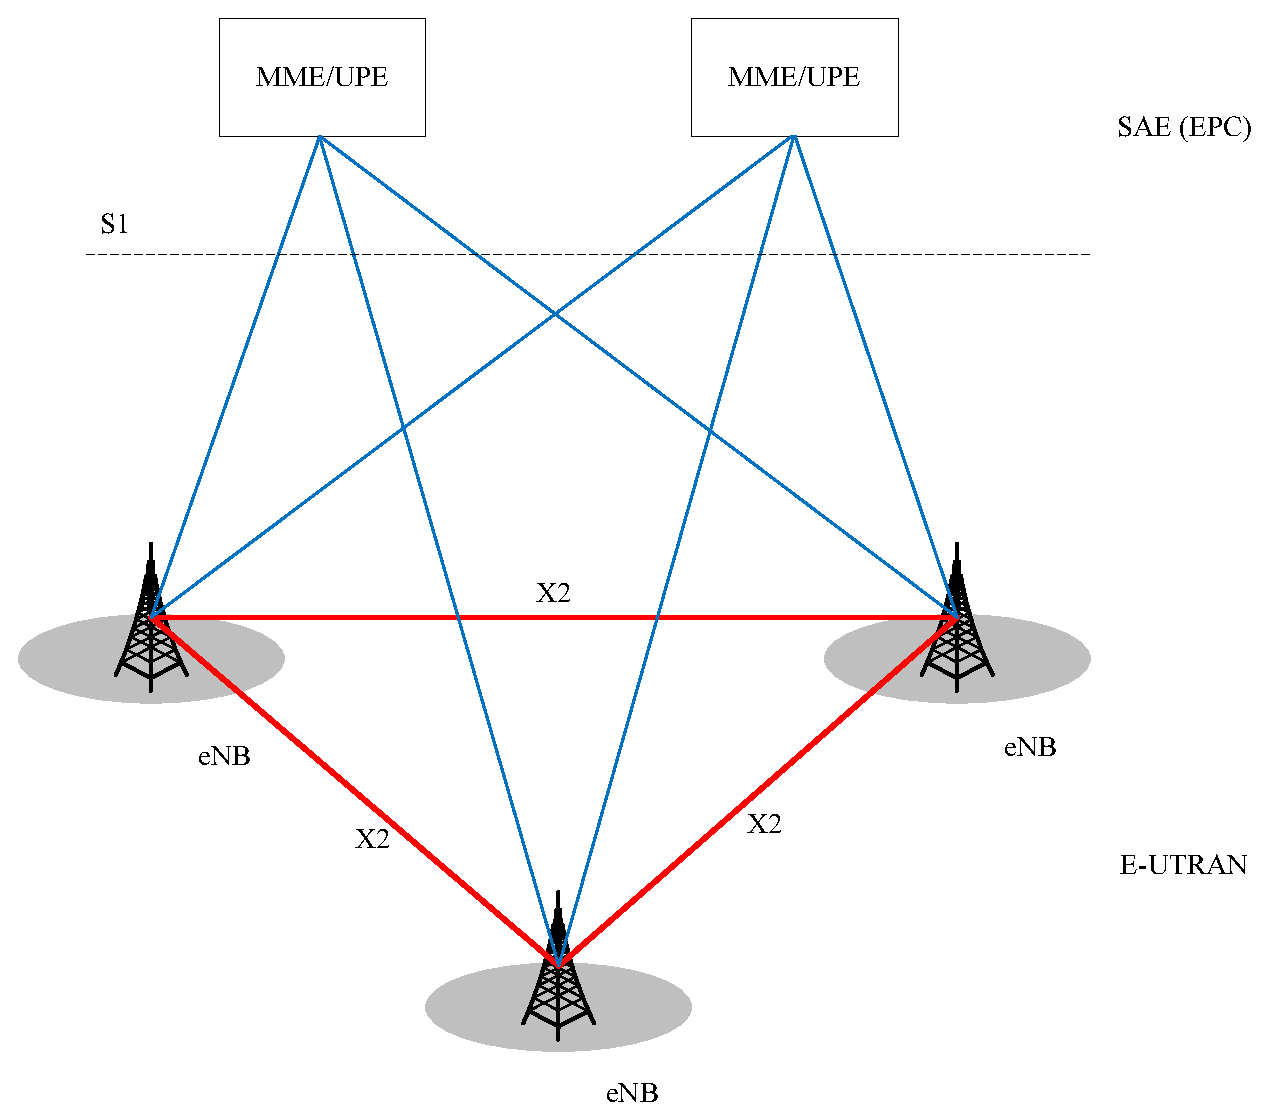
\includegraphics [width=0.8\textwidth] {LTEscheme.eps}
  \caption{Взаимодействие сети радиодоступа E-UTRAN и базовой сети SAE}
  \label{img:LTEscheme}
\end{figure}
Основными требованиями проекта 3GPP к сети SAE были: максимально возможное упрощение структуры сети и исключение дублирующих функций сетевых протоколов, характерных для систем UMTS.
Сети радиодоступа E-UTRAN рассмотрены в ряде технических спецификаций, согласно которым она состоит только из базовых станций eNB (evolved Node B). Базовые станции eNB являются элементами полносвязной сети E-UTRAN и соединены между собой по принципу каждый с каждым при помощи интерфейса X2. Интерфейс X2 поддерживает хендовер мобильного терминала в состоянии LTE\_ACTIVE. Каждая базовая станция имеет интерфейс S1 с базовой сетью SAE, построенная по принципу коммутацая пакетов.
Базовая сеть SAE \cite{lte}, иногда называемая сетью EPC (Evolved Packet Core), содержит узлы MME/UPE, состоящие из логических элементов MME и UPE. Логический элемент MME (Mobility Management Entity) отвечает за решение задач управления мобильностью абонентского терминала и взаимодействует с базовыми станциями eNB сети E-UTRAN с помощью протоколов плоскости управления C-plane (интерфейс S1-C). Логический элемент UPE (User Plane Entity) отвечает за передачу данных пользователей согласно протоколам плоскости пользователя U-Plane и взаимодействует с eNB посредством интерфейса S1-U.
Благодаря интерфейсу S1 базовые станции соединены с несколькими узлами MME/UPE, что позволяет более гибко использовать сетевой ресурс. Такой интерфейс называют S1-flex.
Сеть LTE имеет следующие функциональные отличия от сети UMTS.

\begin{enumerate}
  \item Базовые станции eNB выполняют функции управления радиоресурсами RRM (Radio Resource Management): управление радиоканалами (Radio Bearer Control), управление доступом (Radio Admission Control), управление мобильностью (Connection Mobility Control), динамическое распределение ресурсов (Dynamic Resource Allocation). Таким образом, в сети радиодоступа E-UTRAN базовые станции eNB управляют протоколами радиоинтерфейса, комбинируя выполнение функций базовых станций Node В и большинства функций контроллера RNC сети UMTS.
  \item Сетевой элемент управления мобильностью MME отвечает за распределение сообщений вызова (paging) к базовым станциям eNB. Кроме того, MME управляет протоколами плоскости управления: назначения идентификаторов абонентских терминалов, обеспечения безопасности сети, проверки подлинности сообщений абонентов и управления роумингом.
  \item Сетевой элемент плоскости пользователя UPE выполняет сжатие заголовков IP-протоколов, шифрование потоков данных, терминацию пакетов данных плоскости пользователя, коммутацию пакетов данных при обеспечении мобильности пользователя. Кроме того, UPE управляет протоколами пользовательского уровня, например, хранением текущего статуса абонентского терминала (АТ), прерыванием состояния LET\_IDLE на уровне абонентских терминалов.
\end{enumerate}
Основные протоколы интерфейса S1 плоскостей C-plane и U-plane сети LTЕ представлены на рис. \ref{img:LTEinterface}.
\begin{figure} [h]
  \center
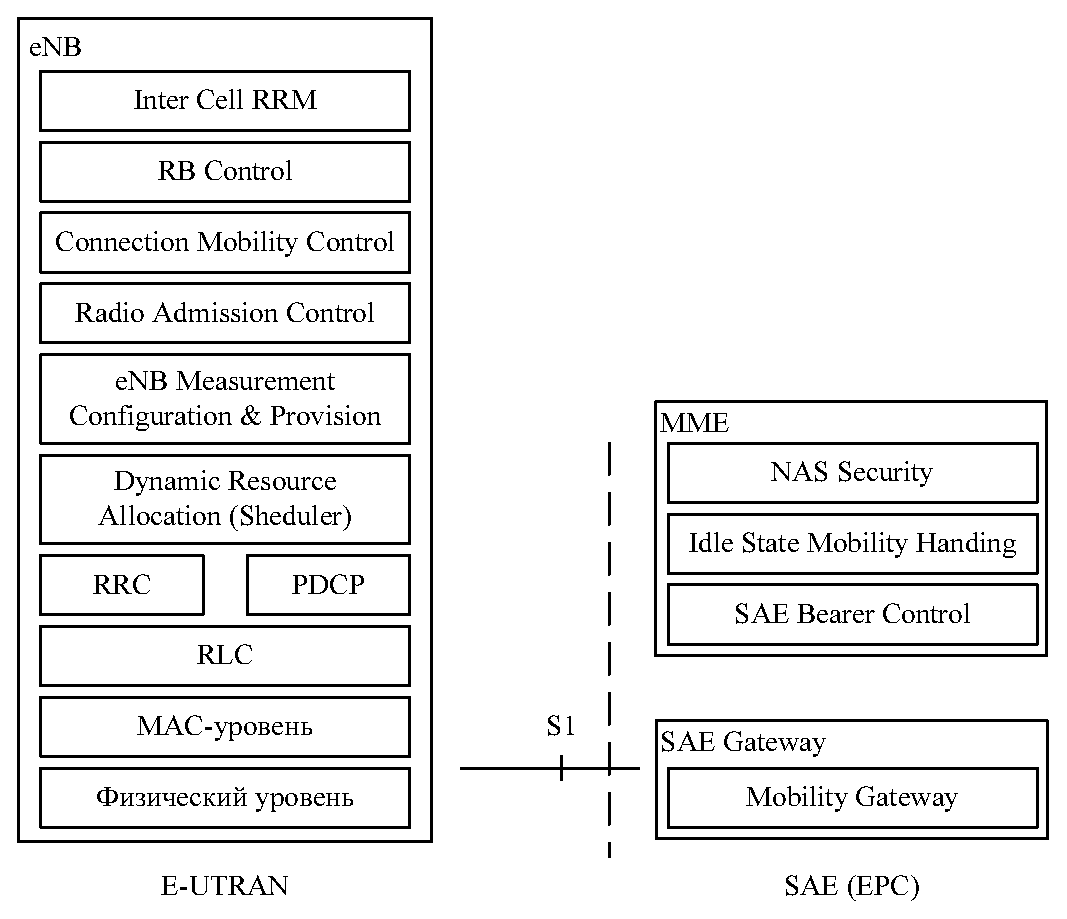
\includegraphics [width=0.6\textwidth] {LTEinterface.eps}
  \caption{Протоколы интерфейса S1 сети LTE}
  \label{img:LTEinterface}
\end{figure}
Одной из важнейших задач управления в сети LTE является максимально эффективное использование радиоресурсов. Данная задача решается с помощью совокупности функций управления радиоресурсами RRM (управление радиоресурсами сети E-UTRAN, управление службой передачи данных в радиоканале, управление мобильностью, управление доступом, динамическое распределение ресурсов) и с помощью протокола управления радиоресурсами RRC. 
Управление радиоресурсами сети E-UTRAN (Inter Cell RRM) обеспечивает управление ресурсами группы сот в целях повышения эффективности использования частотного спектра и минимизации помехового взаимного влияния абонентских терминалов и базовых станций, а также поддержку мобильности.
Управление службой передачи данных в радиоканале (RB Control) реализовано в базовых станциях eNB сети E-UTRAN и обеспечивает установление, поддержание и освобождение радиоканалов передачи данных с заданными параметрами в сети E-UTRAN. Основными задачами являются контроль и управление всеми активными сессиями передачи данных с учетом параметров качества услуг (QoS), выделение ресурсов для вновь активируемых сессий.
Управление мобильностью (Connection Mobility Control) позволяет выбирать обслуживающую базовую станцию eNB для мобильного терминала, передавать обслуживание мобильного терминала от одной базовой станции eNB (хэндовер) к другой. Выбор обслуживающей eNB осуществляется мобильным терминалом на основе собственных измерений в состоянии RRC\_CONNECTED и сравнения полученных измерений с установленными пороговыми значениями. Хэндовер реализован на основе анализа измерений как мобильного терминала, так и базовой станции eNB, а также текущей загрузки обслуживающей и соседних сот, политикой оператора по регулированию трафика.
Поддержку мобильности абонентского терминала в сети SAE обеспечивает логический элемент MME. Основными функциями MME являются:
\begin{itemize}
  \item Управление мобильностью абонентского терминала, находящегося в состоянии RRC\_IDLE (Idle State Mobility Handling).
  \item Управление безопасностью мобильной связи (NAS Security) в соответствии с протоколами, относящимися к группе протоколов «уровня без доступа» и обеспечивающими, например, аутентификацию пользователей, управление ключами шифрования данных.
  \item Управление службой передачи данных сети SAE (SAE Bearer Control).
\end{itemize}
Параметры функций управления радиоресурсами сети E-UTRAN (Inter
Cell RRM), управления службой передачи данных в радиоканале (RB Control) и управления мобильностью (Connection Mobility Control) могут быть кастомизированы в соответствии с требованиями оператора.
Основной задачей по управлению доступом (Radio Admission Control) является формирование решений о предоставлении доступа мобильному терминалу к сети E-UTRAN. Данная задача решается на основе многокритериального анализа загрузки сети радиодоступа, требований мобильного терминала к параметрам QoS.
Динамическое распределение ресурсов (Dynamic Resource Allocation Scheduler) отвечает за планирование очередности передачи пакетов данных и позволяет динамически выделять и перераспределять ресурсы сети радиодоступа, включая канальные ресурсы, мощность излучения базовых станций, ресурсы буферизации при обработке пакетов данных с учетом параметров QoS.
Протокол управления радиоресурсами RRC плоскости С-plane обеспечивает:
\begin{itemize}
  \item Вещание служебной информации в соответствии с протоколами, относящимися к группам протоколов «уровня с доступом» и «уровня без доступа» (соответственно AS - Access Stratum и NAS - Non-Access Stratum).
  \item Пейджинг мобильного терминала.
  \item Установление, поддержание и закрытие RRC-соединений между абонентским терминалом и сетью E-UTRAN.
  \item Управление ключами шифрования.
  \item Установление, поддержание и закрытие служб передачи данных в радиоканале (Radio Bearers) типа «точка-точка» и «точка-многоточка» с заданными параметрами QoS.
  \item Мобильность абонентских терминалов.
\end{itemize}
Кроме того, протокол RRC обеспечивает выполнение ряда других функций.
Протокол сходимости пакетных данных PDCP (Packet Data Convergence Protocol) плоскостей U-plane и C-plane обеспечивает устранение избыточности (сжатие) служебной информации, объем которой может быть соизмерим с объемом полезной информации, передаваемой в пакетах данных, а также шифрование/дешифрование данных.
Протокол управления радиоканалом RLC (Radio Link Control) обеспечивает:
\begin{itemize}
  \item Сегментацию и компоновку пакетов данных протоколов более высокого уровня PDU (Protocol Data Unit) переменной длины в меньшие блоки полезной нагрузки PU (Packet Unit); размер блока PU определяется в соответствии со скоростью передачи информации в радиоканале.
  \item Конкатенцию (сочленение) коротких пакетов PDU верхнего уровня.
  \item Заполнение остатка поля данных блока PU, если сочленение неприемлемо.
  \item Передачу данных пользователя с подтверждением и неподтверждением приема в соответствии с параметрами QoS.
  \item Исправление ошибок методом повторной передачи (ARQ) пакетов данных.
  \item Сохранение на более высоком уровне порядка доставки пакетов PDU при передаче данных с подтверждением приема.
  \item Обнаружение дублирования пакетов PDU для доставки их на более высокий уровень только один раз.
  \item Управление скоростью передачи данных.
  \item Контроль порядковых номеров пакетов.
\end{itemize}


\subsection{Архитектура базовой сети SAE} \label{sect1_2_2}
Архитектура базовой сети SAE позволяет осуществлять дальнейшую эволюцию сетей 3G в направлении получения более высоких скоростей передачи данных, обеспечения низких задержек, а также оптимизации передачи данных на основе разнообразных технологий радиодоступа. Основным отличием базовой сети SAE от базовой сети системы UMTS является максимально упрощенная структура и отсутствие дублирующих функций сетевых протоколов.
Архитектура базовой сети SAE представляет собой PS-домен системы LTE, который предоставляет как услуги передачи речи, так и всю совокупность IP-услуг на основе технологий пакетной коммутации данных. В основу построения базовой сети SAE положена концепция «все через IP» (all-IP или AIPN — All over IP Network) и то обстоятельство, что доступ к базовой сети SAE может осуществляться как через сети радиодоступа второго и третьего поколений (например, сети UTRAN, GERAN), так и через сети радиодоступа не европейских технологий, не стандартизированные проектом 3GPP (сети He-3GPP), например, сети IEEE: Wi-Fi, WiMAX, а также через сети, использующие проводные IP-технологии (например, сети ADSL+, FTTH и др.).
Эталонная архитектура базовой сети SAE с указанием интерфейсов взаимодействия с внешними сетями показана на рис. \ref{img:SAEnetwork}. Согласно этой архитектуре функции протоколов плоскости управления узла SGSN сети UMTS становятся функциями элемента управления мобильностью MME. Функции контроллера RNC, которые не выполняет базовая станция eNB сети E-UTRAN, и функции протоколов плоскости пользователя узлов SGSN и GGSN реализуются модулем UPE и шлюзовым узлом «привязки» 3GPP Anchor сети SAE. Этот узел предназначен для присоединения сетей 2G/3G к сети LTE. В состав SAE входит также шлюзовый узел привязки SAE Anchor, который служит для присоединения к сети SAE сетей стандартов 3GPP (GSM/UMTS) и стандартов нe-3GPP (Wi-Fi и WiMAX). Узлы привязки 3GPP Anchor и SAE Anchor образуют единый узел привязки IASA (Inter Access System Anchor) для присоединения внешних IP-сетей.
Совокупность логических сетевых элементов MME/UPE, IASA, состоящего из узлов SAE Anchor и 3GPP Anchor (рис. \ref{img:SAEnetwork}), образует базовую пакетную сеть (Evolved Packet Core — ЕРС). Данные логические элементы рассматривались в основном на начальных стадиях разработки стандартов сети LTE. Более детальные исследования, направленные на практическую реализацию архитектуры ЕРС, определили новые сетевые элементы: обслуживающий шлюз S-GW (Serving GW) и шлюз взаимодействия с пакетными сетями P-GW (PDN GW), а также логический элемент MME, функционирующий отдельно от элемента UPE. Шлюзы S-GW и Р-GW физически могут быть реализованы в составе одного сетевого элемента AGW (Access GW).
Краткое описание основных интерфейсов сети SAE приведено в табл. \ref{SAEinterface}.
\begin{figure} [h]
  \center
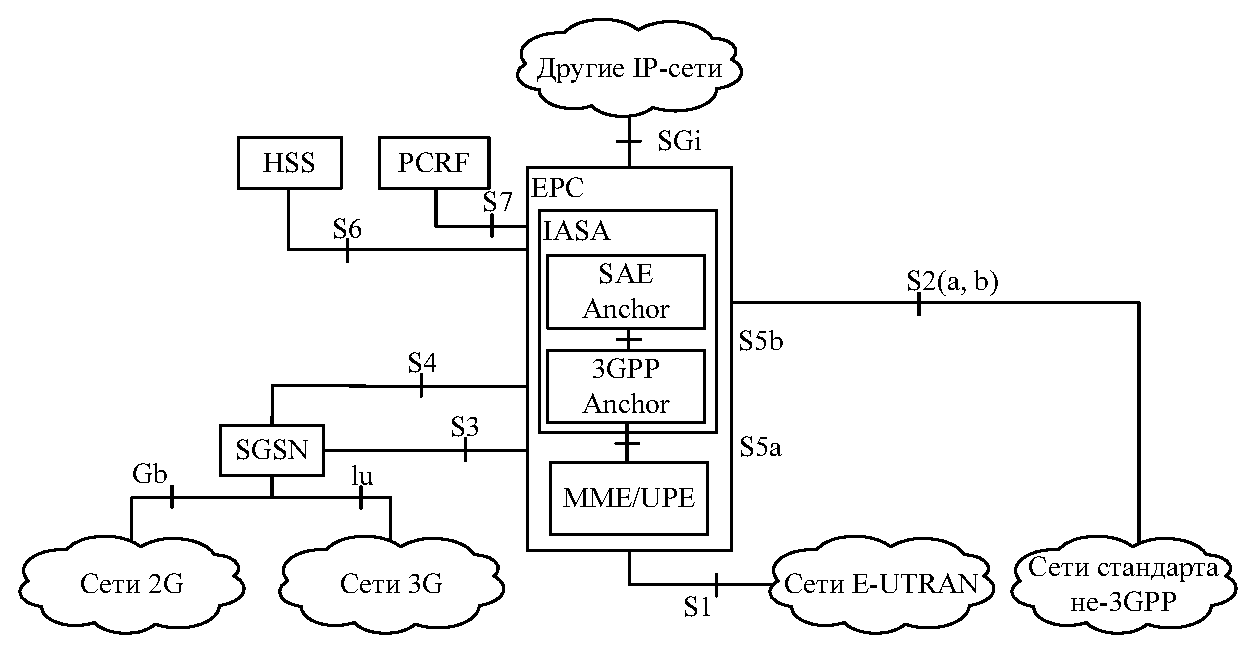
\includegraphics [width=0.95\textwidth] {SAEnetwork.eps}
  \caption{Эталонная архитектура базовой сети SAE}
  \label{img:SAEnetwork}
\end{figure}

\begin{table} [htbp]
  \centering
  \parbox{15cm}{\caption{Основные интерфейсы сети SAE}\label{SAEinterface}}
%  \begin{center}
  \begin{tabular}[t]{| p{3cm} || p{12cm}l |}
  \hline
  \hline
  Интерфейс & \centering  Описание интерфейса & \\
  \hline
  \hline
  S1 & \centering  Интерфейс, предоставляющий доступ к сети радиодоступа E-UTRAN для передачи данных протоколов плоскостей пользователя и управления. Позволяет иметь раздельную и комбинированную аппаратную реализацию элементов MME и UPE & \\
  \hline
  S2a & \centering Интерфейс между узлом IASA и фиксированными IP-сетями стандарта нe-3GPP. Обеспечивает передачу данных протоколов плоскости пользователя и поддержку функций управления и мобильности. Включает в себя интерфейсы S2a, S2b и S2c & \\
  \hline
  S3 & \centering Интерфейс между элементами MME/UPE и узлом SGSN. Обеспечивает управление межсетевым хэндовером абонентских терминалов в сетях E-UTRAN и UTRAN  & \\
  \hline
  S4 & \centering Интерфейс между узлом 3GPP Anchor и узлом SGSN. Обеспечивает передачу данных плоскости пользователя и поддержку функций управления и мобильности. Основан на интерфейсе Gn между узлами SGSN и GGSN сети UMTS  & \\
  \hline
  S5a & \centering Интерфейс между элементом MME/UPE и узлом 3GPP Anchor. Обеспечивает передачу данных протоколов плоскости пользователя и поддержку функций управления и мобильности  & \\
  \hline
  S5b & \centering Интерфейс между узлами 3GPP Anchor и SAE Anchor. Обеспечивает передачу данных протоколов плоскости пользователя и поддержку функций управления и мобильности   & \\
  \hline
  S6 & \centering Интерфейс, обеспечивающий доступ к домашней базе данных пользователей (HSS) для аутентификации и авторизации пользователей (интерфейс ААА) & \\
  \hline
  S7 & \centering Интерфейс, обеспечивающий управление установлением соединений с заданными параметрами QoS на основе политики сети и тарификацию (Policy and Charging Rules Function — PCRF)    & \\
  \hline
  SGi & \centering Интерфейс между узлом IASA и внешними сетями с пакетной передачей данных. Эти сети могут принадлежать как разным операторам, так и одному оператору сотовой связи для предоставления, например, услуг подсистемы IMS. Этот интерфейс основан на интерфейсе Gi между узлами GGSN и внешними IP-сетями  & \\
  \hline
  \hline
  \end{tabular}
%  \end{center}
\end{table}









\section{Предоставление услуг передачи речи и видео поверх LTE (VoLTE)} \label{sect1_4}
\subsection{Предпосылки предоставления услуг передачи речи и видео поверх LTE}


Мобильная связь стандарта LTE оптимизирована для передачи данных и реализована в виде коммутации пакетов через IP. LTE не включает в себя домен с коммутацией каналов, который в настоящее время используется для предоставления услуг передачи речи и SMS услуг. Спрос на услуги мобильного широкополосного доступа растет и операторы запускают высокоскоростные сети на основе технологии LTE. Тем не менее, услуги передачи речи и SMS услуги приносят около 70\% от общей выручки операторов и ясно что эта функциональность должна быть реализована в сетях LTE.

С передачей речи поверх LTE (GSMA VoLTE IR.92 спецификация, основанная на глобальных 3GPP стандартах) абоненты получают возможность голосовых и видео звонков и другие услуги для LTE смартфонов.

Для реализации услуг передачи речи поверх сети LTE, необходимо чтобы IMS  (IP Multimedia System) ядро сети предоставляло сервис телефонии поверх IP. MMTel  (Multi Media Telephony, разработанная в IMS ядре) является решением, которое предоставляет услуги телефонии (включая видео звонки, чат и другое) как в LTE так и в фиксированной сети. LTE сеть радио доступа и EPC также должно поддерживать VoLTE, которое может быть достигнуто обновлением программного обеспечения.

Операторы могут использовать тоже самое ядро сетевой инфраструктуры IMS в VoLTE для развития мобильной и фиксированной конвергенции между любыми устройствами.
Пользователи будут иметь возможность использовать предоставляемые оператором высококачественные голосовые и видео звонки и другие услуги связи на LTE смартфонах и других устройствах.

Эти услуги используют обычный номер мобильного телефона (MSISDN, Mobile Subscriber Integrated Services Digital Network-Number), а VoLTE приносит функции мобильного оператора в мобильную широкополосную сеть основанную на IP. С помощью VoLTE услуги передачи речи данный могут быть использованы одновременно на LTE устройства.


\begin{figure} [h]
  \center
\includegraphics [width=0.95\textwidth] {ericsson/volte1.png}
  \caption{Общий сетевой обзор решения VoLTE (IMS, EPC, LTE), включая поддержку устаревших сетей, когда пользователь находится за пределами покрытия LTE \cite{ericsson_backgrounder}}
  \label{img:volte1}
\end{figure}





Мобильный широкополосный доступ создал целый мир возможностей и открыл новые источники дохода для операторов. Возможности часто сочетаются с проблемами. Решающий вопрос состоит в том, чтобы воспользоваться возможностями широкополосного доступа и в тоже время сохранить и увеличить доходы от услуг связи, таких как передача речи и SMS. Сети LTE могут предоставлять широкополосный доступ и услуги связи с большими возможностями и с меньшей задержкой.  

Некоторые ОТТ (Over the Top) решения, такие как Skype, часто предустановленные на смартфоны, получили широкое распространение. Термин OTT означает доставку видео и аудио сигнала на приставку (компьютер, мобильный телефон) пользователя по сети Интернет без прямого контакта с оператором связи в отличие от услуг VoIP и IPTV, которые предоставляются через управляемую оператором сеть с гарантированным QoS. Тем не менее, ОТТ решения не могут полностью удовлетворить пользователей, так как предоставляются без гарантированного QoS, нет поддержки хэндовера в сеть с коммутацией каналов, нет широкого взаимодействия услуг между различными службами OTT и устройствами, нет поддержки вызова чрезвычайных служб, имеют проблемы с безопасностью. Следовательно, использование сервисов OTT клиентом напрямую зависит от покрытия мобильной широкополосной связи и готовностью абонентами использовать сервис, который испытывает недостаток в качестве, безопасности и гибкости. 

Операторы уже сейчас могут начать глобальное развертывание комерческих решений голосовых и видео звонков поверх LTE - еще до того, когда LTE сеть будет полностью развернута.

LTE и EPC архитектуры не включают поддержку коммутации голосовых и видео звонков. 
Перед началом использования LTE в телефонах, это ограничение должно быть решено. На данный момент существует два решения этой проблемы \cite{ericsson_backgrounder}: CS fallback (CSFB) и IMS/VoLTE. CSFB подходит для использования, когда LTE покрытие является неоднородным (как правило, на ранних этапах развертывания LTE), а IMS/VoLTE может быть реализована, когда покрытие практически однородно (как правило, когда сеть LTE уже в более зрелом состоянии).





\subsection{Обзор системы IP-мультимедиа (IMS)} \label{sect1_3_1}


Подсистема IP-мультимедиа (IMS) разработана отраслевым комитетом 3GPP (3G Partnership Project) для использования IP-ядер в сетях 3G и сейчас применяется объединенным техническим комитетом TISPAN в качестве ключевого элемента инфраструктуры Сетей Следующего Поколения (NGN). IMS – это не только VoIP. Это возможность организации новых мультимедийных сервисов поверх стандартной IP-сети, требующая небольших затрат и позволяющая предоставить услуги абонентам по привлекательным ценам. Производители, выбравшие стратегию развития новых сервисов путем переноса несвязанного между собой частного ПО на одну платформу, не смогут достигнуть такого же уровня интеграции сервисов, развития новых услуг и поддержки клиентов, как поставщики решений, выбравшие стратегию IMS. IMS не только даст возможность пользователю работать с услугами, используя самый широкий спектр клиентских устройств, но и позволит оператору в интересах клиента формировать новые сервисы, используя существующие. Развертывание подсистемы IP-мультимедиа становится ключевым фактором создания комплексных персонализированных услуг. Ожидается, что уже в ближайшем будущем операторы приступят к полному использованию ее возможностей.





На рис. \ref{img:IMS} представлена архитектура IMS, определеная в стандартах 3GPP (3rd Generation Partnership Project) и Европейского института стандартов связи ETSI.
\begin{figure} [h]
  \center
\includegraphics [width=0.95\textwidth] {Imsoverview-2.png}
  \caption{Архитектура IMS}
  \label{img:IMS}
\end{figure}

Унифицированная сервисная архитектура IMS поддерживает широкий спектр сервисов, основанных на гибкости протокола SIP (Session Initiation Protocol). IMS поддерживает множество серверов приложений, предоставляющих как обычные телефонные услуги, так и новые сервисы (обмен мгновенными сообщениями, мгновенная многоточечная связь, передача видеопотоков, обмен мультимедийными сообщениями и т.д.). Сервисная архитектура представляет собой набор логических функций, которые можно разделить на три уровня: уровень абонентских устройств и шлюзов, уровень управления сеансами и уровень приложений.

\textbf{Уровень абонентских устройств и транспорта.}

На этом уровне инициируется и терминируется сигнализация SIP, необходимая для установления сеансов и предоставления базовых услуг, таких как преобразование речи из аналоговой или цифровой формы в IP-пакеты с использованием протокола RTP (Realtime Transport Protocol). На этом уровне функционируют медиашлюзы, преобразующие базовые потоки VoIP в телефонный формат TDM. Медиасервер предоставляет различные медиасервисы, в том числе конференц-связь, воспроизведение оповещений, сбор тоновых сигналов, распознавание речи, синтез речи и т.п. Ресурсы медиасервера доступны всем приложениям, т.е. любое приложение (голосовая почта, бесплатный номер 800, интерактивные VXML-сервисы и т.д.), которому необходимо воспроизвести оповещение или получить цифры набранного номера, может использовать общий сервер. Медиасерверы также поддерживают и нетелефонные функции, например, тиражирование речевых потоков для оказания сервиса мгновенной многоточечной связи (PTT). При использовании для различных сервисов общего пула медиасерверов отпадает необходимость в планировании и инжиниринге медиаресурсов для каждого отдельного приложения.


\textbf{Уровень управления вызовами и сеансами.}

На этом уровне располагается функция управления вызовами и сеансами CSCF (Call Session Control Function), которая регистрирует абонентские устройства и направляет сигнальные сообщения протокола SIP к соответствующим серверам приложений. Функция CSCF взаимодействует с уровнем транспорта и доступа для обеспечения качества обслуживания по всем сервисам. Уровень управления вызовами и сеансами включает сервер абонентских данных HSS (Home Subscriber Server), где централизованно хранятся уникальные сервисные профили всех абонентов. Профиль содержит текущую регистрационную информацию (например, IP-адрес), данные роуминга, данные по телефонным услугам (например, номер переадресации), данные по обмену мгновенными сообщениями (список абонентов), параметры голосовой почты (например, приветствия) и т.д. Централизованное хранение позволяет различным приложениям использовать эти данные для создания персональных справочников, информации о присутствии в сети абонентов различных категорий, а также совмещенных услуг. Централизация также существенно упрощает администрирование пользовательских данных и гарантирует однородное представление активных абонентов по всем сервисам.

На уровне управления вызовами и сеансами также располагается функция управления медиашлюзами MGCF (Media Gateway Control Function), которая обеспечивает взаимодействие сигнализации SIP с сигнализацией других медиашлюзов (например, H.248). Функция MGCF управляет распределением сеансов по множеству медиашлюзов, для медиасерверов это выполняется функцией MSFC (Media Server Function Control).

\textbf{Уровень серверов приложений.}

Этот уровень содержит серверы приложений, которые обеспечивают обслуживание конечных пользователей. Архитектура IMS и сигнализация SIP обеспечивают достаточную гибкость для поддержки разнообразных телефонных и других серверов приложений. Так, разработаны стандарты SIP для сервисов телефонии и сервисов IM.



\subsection{Предоставление услуг передачи речи и видео поверх LTE на основе CSFB}

Стандартизированным решением для предоставления услуг передачи речи в начале развертывания LTE, является CSFB \cite{ericsson_volte}. При использовании, устройства перенаправленные на WCDMA/GSM (рис. \ref{img:csfb}) для инициализации или приема голосовых сообщений, остаются в области CS, пока не будут завершены. CSFB предоставляет поддержку услуг передачи речи и SMS, и считается первым шагом в эволюции направленной предоставление мультимедийных услуг связи.

\begin{figure} [h]
  \center
\includegraphics [width=0.95\textwidth] {ericsson/csfb.png}
  \caption{CSFB \cite{ericsson_volte}}
  \label{img:csfb}
\end{figure}







\subsection{Предоставление услуг передачи речи и видео поверх LTE на основе IMS/VoLTE}

Термин передача речи поверх LTE (VoLTE) используется для описания GSMA спецификацию \cite{ir92} для предоставления услуг передачи речи и  SMS в LTE, которая берет свое начало с 3GPP IMS-based multimedia telephony (MMTel) решения. С MMTel операторы могут развивать свои голосовые и мультимедийные сервисы, такие как видео звонки — описанные в спецификации GSMA для IMS видео связи \cite{ir94}. 

Хотя MMTel лежит в основе решения VoLTE, EPC  и LTE  являются неотъемлемой частью его. Вместе они обеспечивают совместимость на всех интерфейсах между устройствами и сетями. Рис. \ref{img:mmtel} иллюстрирует важность принятия сквозного подхода к реализации передачи речи в LTE, для обеспечения классических телекоммуникационных принципов, таких как наивысшие требования QoS к передачи речи (LTE), управление мобильностью (EPC), использование MSISDN для обеспечения глобальной совместимости и различных видов нормативных и дополнительных услуг (IMS и MMTel).


\begin{figure} [h]
  \center
\includegraphics [width=0.95\textwidth] {ericsson/mmtel.png}
  \caption{VoLTE интерфейсы через пользовательский сетевой интерфейс (UNI) между устройством и сетью \cite{ericsson_volte}}
  \label{img:mmtel}
\end{figure}



VoLTE включает передачу речи с полудуплексном режиме с форматом связи точка-точка или точка-многоточка. На рис. \ref{img:voice} показана упрощенная версия VoLTE архитектуры связи.

\begin{figure} [!h]
  \center
\includegraphics [width=0.95\textwidth] {ericsson/voice.png}
  \caption{VoLTE (упрощенный вид) \cite{ericsson_volte}}
  \label{img:voice}
\end{figure}


Когда устройство включается, оно прикрепляется к LTE/EPC сети и применяет IMS Access Point Name (APN) для облегчения роуминга и для получения ссылки на домен IMS, а также для выделения канала для SIP сигнализации (рис. \ref{img:ims_conn}). Затем устройство инициализирует процесс регистрации в домене IMS с идентификатором MMTel и опционально SMS-over-IP идентификатором. Во время этого процесса устройство будет проходить проверку подлинности.



\begin{figure} [!h]
  \center
\includegraphics [width=0.95\textwidth] {ericsson/imsconn.png}
  \caption{Регистрация и аутентификация устроства \cite{ericsson_volte}}
  \label{img:ims_conn}
\end{figure}

Сигнал INVITE содержит Session Description Protocol (SDP), который описывает желаемую среду передачи , и содержит такую информацию, как стандарт кодирования htxb  - Adaptive Multi-Rate Wideband (AMR-WB, используемый для HD речи) или Adaptive Multi-Rate Narrowband (AMR-NB) - IP  адрес и порт для использования. Домен IMS передает эту информацию через стандартизированные интерфейсы в EPC’s Policy и Charging Enforcement Function (PCEF), которые в свою очередь выполняют QoS требования и анализ загруженных правил. Типичный результат этого анализа может быть - выделение EPC и радиоканала для данных - с гарантированной скоростью передачи VoIP среды. Рис. \ref{img:voice1} иллюстрирует SIP сигнализацию и речевой поток по выделенному каналу.

\begin{figure} [!h]
  \center
\includegraphics [width=0.95\textwidth] {ericsson/voice1.png}
  \caption{Канал для передачи сигнальной информации и канал для передачи речи \cite{ericsson_volte}}
  \label{img:voice1}
\end{figure}

Технология LTE создала огромное количество возможностей, но возможности часто сочетаются с проблемами. 
Услуги реального времени, которые позволяет внедрять технология VoLTE (такие как голосовые звонки в HD качестве, видео звонки, организация конференций с эффектом присутствия и т. д.) критичны к джиттеру задержки. 
Беспроводные сети LTE и проводные сети, которые соединяют LTE сеть с контент серверами или другими беспроводными сетями, подвержены задержке, джиттеру и потери пакетов. 
Далее рассмотрим основные требования QoS к предоставлению голосовых и видео потоковых сервисов.
\section{Анализ требований QoS для предоставления сервисов передачи данных, голоса и видео } \label{sect_qos}

Основными факторами,  влияющими на качество передачи голоса в IP  сетях,  являются задержка передачи и процент потери пакетов [1].
На рис. \ref{img1:qos_dd} показаны контуры качества передачи речи (удовлетворенности пользователя) для кодека G.711 с включенной функцией скрытия потерь пакетов (PLC).

\pgfplotsset{width=15cm, height=10cm, compat=1.3}
\begin{figure} [h]
  \center
\begin{tikzpicture}
\pgfkeys{ /pgf/number format/.cd,
        use comma,
        1000 sep={}}
\pgfkeys{/pgfplots/legend pos=north west}
\begin{axis}[
legend cell align=left,
cycle list name=mark list,
xlabel=Задержка (мс),
ylabel=Пакетные потери (\%),
xmin=0,
xmax=500,
ymax=20,
ymin=0,
]
\node
	at (50,6) {\scriptsize Очень довольны};
\node
	at (70,25) {\scriptsize Пользователи довольны};
\node
	at (100,60) {\scriptsize Некоторые пользователи довольны};
\node
	at (100,100) {\scriptsize Многие пользователи не довольны};
\node
	at (105,160) {\scriptsize Почти все пользователи не довольны};
\node
	at (400,160) {\scriptsize Не рекомендуется};
\addplot[mark=none] coordinates
{(0,1.1) (159,1.1) (205,0)};
\addplot[mark=none] coordinates
{(0,4.1) (159,4.1) (175,3.9) (285,0)};
\addplot[mark=none] coordinates
{(0,8.1) (175,8.1) (265,4.2) (390,0)};
\addplot[mark=none] coordinates
{(0,13.5) (175,13.5) (500,1)};
\addplot[mark=none] coordinates
{(0,20) (200,20) (500,4)};

\end{axis}
\end{tikzpicture}
\caption{Контуры качества передачи речи G711 c PLC}
  \label{img1:qos_dd}
\end{figure}



Наибольший вклад в задержку и потери пакетов вносит не оптимальный буфер компенсации джиттера. 

На рис. \ref{img1:qos_dd} видно, что качество передачи
речи уменьшается с увеличением задержки и
процента потери пакетов. Необходимо определить составляющие, которые вносят
наибольший вклад в задержку и потерю пакетов.
Составляющие задержки при передаче го-
лоса средствами VoIP:
\begin{enumerate}
 \item Аналого-цифровое и цифро-аналоговое преобразование сигнала.
 \item Кодирование/компрессия и декодирование/декомпрессия.
 \item Упаковка блока данных и распаковка блока данных стека протоколов TCP/IP.
 \item Буфер компенсации джиттера.
\end{enumerate}

Для большинства оконечных устройств, работающих с VoIP, потерями на аналого-цифровое и цифро-аналоговое преобразование, 
декодирование/декомпрессию и формирование стека протоколов TCP/IP можно пренебречь. 
Средняя величина задержки, вносимой каждой из составшихся составляющих VoIP \cite{G114,Y1541}, представлена в табл 1.


{%
\newcommand{\mc}[3]{\multicolumn{#1}{#2}{#3}}
\begin{center}
\begin{tabular}[t]{| p{12cm} | p{3cm} |}\hline \hline
\mc{1}{|c|}{Наименование} & \mc{1}{c|}{Вносимая задержка}\\ \hline \hline
Оптический кабель & 5 мкс/км\\ \hline
Система наземной мобильной связи & 80-110 мс\\ \hline 
Кодек G.729 для 20 мс блоков & 25 мс\\ \hline
Кодек GSM для 20 мс блоков & 20 мс\\ \hline
Сетевое оборудование (L3), суммарное время нахождения в очереди и обработка & 2-10 мс на узел\\ \hline
Буфер компенсации джиттера & 20-60 мс\\ \hline
\end{tabular}
\end{center}
}%

В соответствии с рекомендациями \cite{G114} максимальная задержка при передаче голоса в одну сторону не должна превы-шать 150 мс.
Таким образом, в зависимости от параметров сети, до 40\% допустимой задержки может составлять задержка в буфере компенсации джиттера.
Буфер компенсации джиттера компенсирует отклонения значений задержки от среднего значения. Прибывающие пакеты на приемной стороне
воспроизводятся не сразу, а с определенной задержкой. Чем больше джиттер, тем больше размер буфера требуется для компенсации изменений задержки, иначе часть пакетов будет отброшена, если они придут позже времени воспроизведения. 
При максимальном размере буфера появляется возможность свести количество отбрасываемых пакетов к минимуму, но при этом увеличивается время задержки. 
При минимальном размере буфера время задержки уменьшается, но при этом увеличивается количество отбрасываемых пакетов.

Следовательно, размер буфера должен меняться во времени по алгоритму, учитывающему текущее состояние сети. 
И чем динамичнее алгоритм, тем выше качество предоставляемого потокового сервиса на приемной стороне. 
Поэтому возникает задача: разработать алгоритм адаптивного управления буфером компенсации джиттера.









\clearpage
\section{Выводы по \ref{chapt1} разделу } \label{sect_conclus1}

\begin{enumerate}
\item Согласно прогнозу \cite{ericsson} 60\% людей в конце 2018 года будут иметь широкополосное мобильное покрытие LTE. Поэтому развитие и оптимизация технологии LTE, на сегодня является актуальной задачей.

\item Сети LTE с помощью технологии VoLTE, позволяют предоставлять услуги реального времени, такие как голосовые звонки в HD качестве, видео звонки, организация конференций с эффектом присутствия и т. д., которые критичны к джиттеру задержки. Беспроводные сети LTE и проводные сети, через которые передаются пакеты этих услуг, могут быть подвержены различным факторам, которые увеличивают джиттер задержки. Поэтому для разработки методов борьбы с джиттером задержки и соответственно улучшения качества предоставления услуг реального времени в сетях LTE, в разделе \ref{chapt2} будут рассмотрены основные факторы, влияющие на джиттер задержки.

\item Сервисы реального времени с повышенной степенью взаимодействия критичны к джиттеру и задержке. В следствие, чего необходимо решить проблему нерационального внесения задержки буфером компенсации джиттера. 
Предложено разработать адаптивноый буфер компенсации джиттера, котрый бы учитывал текущее состояние сети. 
А также разработать способ его внедрения  в сети LTE.

\end{enumerate}

\clearpage




